% questions.tex —— 2006 年·普通高等学校招生考试·陕西卷文科 · 题目内容片段（无答案）
% 由 tools/generate_projects.py 依来源总账自 2006/2006_数学真题_陕西文_试题.md 生成，勿手改（改源 MD 后重跑）


\begin{gktip}
\textbf{来源边界}：据固定候选 PDF 逐题转录，现场 SHA-256 与来源清单记录一致。题签支持卷名与科类的字面记录，但不能认证发布者、出版者、版次、扫描/重排来源链或官方原件身份。固定 PDF 仅见题面，未见答案、解析或评分标准，官方答案未录入。
\textbf{源页定位}：PDF 第 1 页（印刷页 326）含 Q1–Q19；第 2 页（印刷页 327）含 Q20–Q22。选择题 Q1–Q12，填空题 Q13–Q16，解答题 Q17–Q22。
\textbf{转录说明}：题面文字已与固定 PDF 原页逐题核对；文字层仅作定位候选。按原页保留字母、公式、条件与选项，不按题意推断修正。题图已依据固定候选 PDF 原页重绘为本卷 TikZ 源并链接；独立预览已检查，正式 TeX 构建与逐页视觉验收仍待完成。
\end{gktip}

\gkpart{一、选择题}

\begin{question}
\gkti{1}
已知集合 \(P=\{x\in\mathbb N\mid 1\le x\le10\}\)，集合 \(Q=\{x\in\mathbb R\mid x^2+x-6=0\}\)，则 \(P\cap Q\) 等于（ ）。

(A) \(\{2\}\)　(B) \(\{3\}\)　(C) \(\{-2,3\}\)　(D) \(\{-3,2\}\)

\end{question}
\begin{question}
\gkti{2}
函数 \(f(x)=\dfrac{1}{1+x^2}\)（\(x\in\mathbb R\)）的值域是（ ）。

(A) \((0,1)\)　(B) \((0,1]\)　(C) \([0,1)\)　(D) \([0,1]\)

\end{question}
\begin{question}
\gkti{3}
已知等差数列 \(\{a_n\}\) 中，\(a_1+a_8=8\)，则该数列前 9 项和 \(S_9\) 等于（ ）。

(A) 18　(B) 27　(C) 36　(D) 45

\end{question}
\begin{question}
\gkti{4}
设函数 \(f(x)=\log_a(x+b)\)（\(a>0，a\ne1\)）的图象过点 \((0,0)\)，其反函数的图象过点 \((1,2)\)，则 \(a+b\) 等于（ ）。

(A) 6　(B) 5　(C) 4　(D) 3

\end{question}
\begin{question}
\gkti{5}
设直线过点 \((0,a)\)，其斜率为 1，且与圆 \(x^2+y^2=2\) 相切，则 \(a\) 的值为（ ）。

(A) \(\pm\sqrt2\)　(B) \(\pm2\)　(C) \(\pm2\sqrt2\)　(D) \(\pm4\)

\end{question}
\begin{question}
\gkti{6}
“\(\alpha，\beta，\gamma\) 成等差数列”是“等式 \(\sin(\alpha+\gamma)=\sin2\beta\) 成立”的（ ）。

(A) 充分而不必要条件　(B) 必要而不充分条件
(C) 充分必要条件　(D) 既不充分也不必要条件

\end{question}
\begin{question}
\gkti{7}
设 \(x，y\) 为正数，则 \((x+y)\left(\dfrac1x+\dfrac4y\right)\) 的最小值为（ ）。

(A) 6　(B) 9　(C) 12　(D) 15

\end{question}
\begin{question}
\gkti{8}
\Needspace{5\baselineskip}
已知非零向量 \(\overrightarrow{AB}\) 与 \(\overrightarrow{AC}\) 满足
\nopagebreak[4]
\[
\left(\frac{\overrightarrow{AB}}{|\overrightarrow{AB}|}+\frac{\overrightarrow{AC}}{|\overrightarrow{AC}|}\right)\cdot\overrightarrow{BC}=0
\quad\text{且}\quad
\frac{\overrightarrow{AB}}{|\overrightarrow{AB}|}\cdot\frac{\overrightarrow{AC}}{|\overrightarrow{AC}|}=\frac12，
\]
则 \(\triangle ABC\) 为（ ）。

(A) 三边均不相等的三角形　(B) 直角三角形
(C) 等腰非等边三角形　(D) 等边三角形

\end{question}
\begin{question}
\gkti{9}
已知函数 \(f(x)=ax^2+2ax+4\)（\(a>0\)）。若 \(x_1<x_2，x_1+x_2=0\)，则（ ）。

(A) \(f(x_1)<f(x_2)\)　(B) \(f(x_1)=f(x_2)\)
(C) \(f(x_1)>f(x_2)\)　(D) \(f(x_1)\) 与 \(f(x_2)\) 的大小不能确定

\end{question}
\begin{question}
\gkti{10}
已知双曲线 \(\dfrac{x^2}{a^2}-\dfrac{y^2}{2}=1\)（\(a>\sqrt2\)）的两条渐近线的夹角为 \(\dfrac\pi3\)，则双曲线的离心率为（ ）。

(A) 2　(B) \(\sqrt3\)　(C) \(\dfrac{2\sqrt6}{3}\)　(D) \(\dfrac{2\sqrt3}{3}\)

\end{question}
\begin{question}
\gkti{11}
已知平面 \(\alpha\) 外不共线的三点 \(A，B，C\) 到 \(\alpha\) 的距离都相等，则正确的结论是（ ）。

(A) 平面 \(ABC\) 必平行于 \(\alpha\)
(B) 平面 \(ABC\) 必与 \(\alpha\) 相交
(C) 平面 \(ABC\) 必不垂直于 \(\alpha\)
(D) 存在 \(\triangle ABC\) 的一条中位线平行于 \(\alpha\) 或在 \(\alpha\) 内

\end{question}
\begin{question}
\gkti{12}
为确保信息安全，信息需加密传播，发送方由明文 \(\to\) 密文（加密），接收方由密文 \(\to\) 明文（解密）。已知加密规则为：明文 \(a，b，c，d\) 对应密文 \(a+2b，2b+c，2c+3d，4d\)。例如，明文 1，2，3，4 对应密文 5，7，18，16。当接收方收到密文 14，9，23，28 时，则解密得到的明文为（ ）。

(A) 1，6，4，7　(B) 4，6，1，7　(C) 7，6，1，4　(D) 6，4，1，7

\end{question}
\gkpart{二、填空题}

\begin{question}
\gkti{13}
\(\cos43^\circ\cos77^\circ+\sin43^\circ\cos167^\circ\) 的值为 \gkblank{}。

\end{question}
\begin{question}
\gkti{14}
\(\left(2x-\dfrac1{\sqrt{x}}\right)^6\) 展开式中的常数项为 \gkblank{}。（用数字作答）

\end{question}
\begin{question}
\gkti{15}
某校从 8 名教师中选派 4 名教师同时去 4 个边远地区支教（每地 1 人），其中甲和乙不同去，则不同的选派方案共有 \gkblank{} 种。

\begin{gktip}
原页原文“甲和乙不同去”照录；本阶段不按推测解释该选派条件。
\end{gktip}

\end{question}
\begin{question}
\gkti{16}
水平桌面 \(\alpha\) 上放有 4 个半径均为 \(2R\) 的球，且相邻的球都相切（球心的连线构成正方形）。在这 4 个球的上面放 1 个半径为 \(R\) 的小球，它和下面的 4 个球恰好都相切，则小球的球心到水平桌面 \(\alpha\) 的距离是 \gkblank{}。

\end{question}
\gkpart{三、解答题}

\begin{question}
\gkti{17}
甲、乙、丙 3 人投篮，投进的概率分别是 \(\dfrac25，\dfrac12，\dfrac35\)。现 3 人各投篮 1 次，求：

(1) 3 人都投进的概率；
(2) 3 人中恰有 2 人投进的概率。

\end{question}
\begin{question}
\gkti{18}
已知函数 \(f(x)=\sqrt3\sin\left(2x-\dfrac\pi6\right)+2\sin^2\left(x-\dfrac\pi{12}\right)\)（\(x\in\mathbb R\)）。

(1) 求函数 \(f(x)\) 的最小正周期；
(2) 求使函数 \(f(x)\) 取得最大值的 \(x\) 的集合。

\Needspace{0.4\textheight}
\end{question}
\begin{question}
\gkti{19}
如图，\(\alpha\perp\beta，\alpha\cap\beta=l，A\in\alpha，B\in\beta\)，点 \(A\) 在直线 \(l\) 上的射影为 \(A_1\)，点 \(B\) 在 \(l\) 上的射影为 \(B_1\)。已知 \(AB=2，AA_1=1，BB_1=\sqrt2\)。求：

(1) 直线 \(AB\) 分别与平面 \(\alpha，\beta\) 所成角的大小；
(2) 二面角 \(A_1-AB-B_1\) 的大小。
\nopagebreak[4]
\begin{center}% Source-faithful schematic draft: src-d3bb569fc2c589e075c748b1494aaadeaae67bbe0e3926306e123e08de2a5fec
% Source SHA-256 ef53636f75f8cef48067ff22478f699a5ac7d3dee4a42f06e01e640bc906d221; PDF p.1, Q19.
% Diagram topology only; no measurements, angle, or additional incidence claims beyond visible projections.
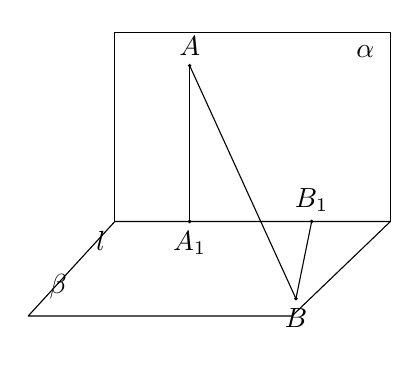
\begin{tikzpicture}[line join=round, line cap=round]
  % Plane alpha, shown as a vertical parallelogram, and its lower edge l.
  \draw (0,0) -- (3.5,0) -- (3.5,2.4) -- (0,2.4) -- cycle;
  \node at (3.18,2.16) {$\alpha$};
  % Plane beta, shown receding below l; shared edge is the intersection l.
  \draw (0,0) -- (3.5,0) -- (2.25,-1.2) -- (-1.1,-1.2) -- cycle;
  \node at (-0.72,-0.83) {$\beta$};
  \node[below left] at (0,0) {$l$};
  % A and B with their visible projections A_1 and B_1 onto l.
  \coordinate (A) at (0.95,1.98);
  \coordinate (Aone) at (0.95,0);
  \coordinate (B) at (2.30,-0.98);
  \coordinate (Bone) at (2.50,0);
  \draw (A)--(B);
  \draw (A)--(Aone);
  \draw (B)--(Bone);
  \fill (A) circle (0.7pt) node[above] {$A$};
  \fill (B) circle (0.7pt) node[below] {$B$};
  \fill (Aone) circle (0.7pt) node[below] {$A_1$};
  \fill (Bone) circle (0.7pt) node[above] {$B_1$};
\end{tikzpicture}
\end{center}
\nopagebreak[4]
\end{question}
\begin{question}
\gkti{20}
已知正项数列 \(\{a_n\}\)，其前 \(n\) 项和 \(S_n\) 满足 \(10S_n=a_n^2+5a_n+6\)，且 \(a_1，a_3，a_{15}\) 成等比数列，求数列 \(\{a_n\}\) 的通项 \(a_n\)。

\Needspace{0.4\textheight}
\end{question}
\begin{question}
\gkti{21}
\Needspace{5\baselineskip}
如图，三定点 \(A(2，1)，B(0，-1)，C(-2，1)\)，三动点 \(D，E，M\) 满足
\nopagebreak[4]
\[
\overrightarrow{AD}=t\overrightarrow{AB}，\quad \overrightarrow{BE}=t\overrightarrow{BC}，\quad \overrightarrow{DM}=t\overrightarrow{DE}，\quad t\in[0，1]\mbox{。}
\]
(1) 求动直线 \(DE\) 斜率的变化范围；
(2) 求动点 \(M\) 的轨迹方程。
\nopagebreak[4]
\begin{center}% Source-faithful schematic draft: src-d3bb569fc2c589e075c748b1494aaadeaae67bbe0e3926306e123e08de2a5fec
% Source SHA-256 ef53636f75f8cef48067ff22478f699a5ac7d3dee4a42f06e01e640bc906d221; PDF p.2, Q21.
% Schematic parameter t=0.4 illustrates AD=t AB, BE=t BC, DM=t DE; this is not an extra value imposed by the source question.
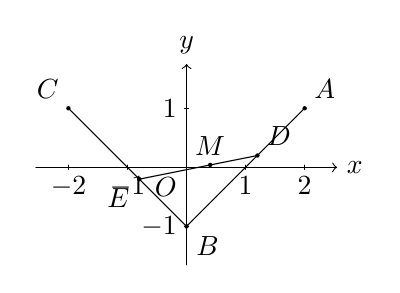
\begin{tikzpicture}[line cap=round, line join=round, x=0.75cm, y=0.75cm]
  \draw[->] (-2.55,0)--(2.55,0) node[right] {$x$};
  \draw[->] (0,-1.65)--(0,1.75) node[above] {$y$};
  \draw (-2,1)--(0,-1)--(2,1);
  \coordinate (A) at (2,1); \coordinate (B) at (0,-1); \coordinate (C) at (-2,1);
  % D and E lie on the two visible sides; M lies on the segment DE.
  \coordinate (D) at (1.2,0.2); \coordinate (E) at (-0.8,-0.2);
  \coordinate (M) at (0.4,0.04);
  \draw (D)--(E);
  \foreach \P/\label/\pos in {A/A/above right,B/B/below right,C/C/above left,D/D/above right,E/E/below left,M/M/above} {
    \fill (\P) circle (0.8pt) node[\pos] {$\label$};
  }
  \node[below left] at (0,0) {$O$};
  \node[below] at (0,-1) {};
  \foreach \xv in {-2,-1,1,2} {\draw (\xv,0.035)--(\xv,-0.035);}
  \foreach \yv in {-1,1} {\draw (0.035,\yv)--(-0.035,\yv);}
  \node[below] at (-2,0) {$-2$}; \node[below] at (-1,0) {$-1$};
  \node[below] at (1,0) {$1$}; \node[below] at (2,0) {$2$};
  \node[left] at (0,1) {$1$}; \node[left] at (0,-1) {$-1$};
\end{tikzpicture}
\end{center}
\nopagebreak[4]
\end{question}
\begin{question}
\gkti{22}
设函数 \(f(x)=kx^3-3x^2+1\)（\(k\ge0\)）。

(1) 求函数 \(f(x)\) 的单调区间；
(2) 若函数 \(f(x)\) 的极小值大于 0，求 \(k\) 的取值范围。

\end{question}